\let\negmedspace\undefined
\let\negthickspace\undefined
\documentclass[journal]{IEEEtran}
\usepackage[a5paper, margin=10mm, onecolumn]{geometry}
%\usepackage{lmodern} % Ensure lmodern is loaded for pdflatex
\usepackage{tfrupee} % Include tfrupee package

\setlength{\headheight}{1cm} % Set the height of the header box
\setlength{\headsep}{0mm}  % Set the distance between the header box and the top of the text

\usepackage{gvv-book}
\usepackage{gvv}
\usepackage{cite}
\usepackage{amsmath,amssymb,amsfonts,amsthm}
\usepackage{algorithmic}
\usepackage{graphicx}
\usepackage{textcomp}
\usepackage{xcolor}
\usepackage{txfonts}
\usepackage{listings}
\usepackage{enumitem}
\usepackage{mathtools}
\usepackage{gensymb}
\usepackage{comment}
\usepackage[breaklinks=true]{hyperref}
\usepackage{tkz-euclide} 
\usepackage{listings}
% \usepackage{gvv}                                        
\def\inputGnumericTable{}                                 
\usepackage[latin1]{inputenc}                                
\usepackage{color}                                            
\usepackage{array}                                            
\usepackage{longtable}                                       
\usepackage{calc}                                             
\usepackage{multirow}                                         
\usepackage{hhline}                                           
\usepackage{ifthen}                                           
\usepackage{lscape}
\begin{document}

\bibliographystyle{IEEEtran}
\vspace{3cm}

\title{10.4.3.9}
\author{EE24BTECH11015 - Dhawal}

% \maketitle
% \newpage
% \bigskip
{\let\newpage\relax\maketitle}

\renewcommand{\thefigure}{\theenumi}
\renewcommand{\thetable}{\theenumi}
\setlength{\intextsep}{10pt} % Space between text and floats

\textbf{Question:}

Two water taps together can fill a tank in $\frac{75}{8}$
hours. The tap of larger diameter takes $10$
hours less than the smaller one to fill the tank separately. Find the time in which each tap can separately fill the tank.\\

\textbf{Solution}\\
Let time taken by each tap $A,B$ to fill the tank be $x,y$ respectively.\\
As tap $A$ takes $10$ hours less to fill the tank.
\begin{align}
    y&=x+10
\end{align}
As total time taken by both to fill the tank is $\frac{75}{8}$
\begin{align}
    \brak{\frac{1}{x}+\frac{1}{y}}\frac{75}{8}&=1\\
    \frac{1}{x}+\frac{1}{y}&=\frac{8}{75}
\end{align}
Putting Eq. $1$ in Eq. $3$, we get
\begin{align}
    \frac{1}{x}+\frac{1}{x+10}&=\frac{8}{75}\\
    \frac{2x+10}{x\brak{x+10}}&=\frac{8}{75}\\
    4x^2-35x-375&=0
\end{align}
\textbf{Theoretical Solution}\\
Using quadratic formula, $a=4, b=-35, c=-375$.\\
\begin{align}
    x&=\frac{-b\pm\sqrt{b^2-4ac}}{2a}
\end{align}
We get $x=15$ and $x=-6.25$\\
We can't take negative values so $x=15$ and $y=25$ is the solution.\\\\
So, time taken by each tap $A,B$ to fill the tank is $15,25$ hours.\\

\textbf{Computational Solution}\\
\textbf{Newton's Method}

We will use Newton's Method for solving equations.
\begin{align}
	x_{n+1} = x_n - \frac{f\brak{x_n}}{f^{\prime}\brak{x_n}} 
\end{align}
Where we define $f\brak{x}$ as, 
\begin{align}
	f\brak{x} = 4x^2 - 35x - 375 \\
	f^{\prime}\brak{x} = 8x -35 
\end{align}
Thus, the new update equation is, 
\begin{align}
	x_{n+1} = x_n - \frac{4x^2 - 35x - 375}{8x -35} 
\end{align}
This is a quadratic equation, it can have 2 solutions. As at $x=0,f\brak{x} \leq 0$. So we will iterate it from $ \brak{-100,0} $ and $\brak{0,100}$. Take initial guess as $x_0 = 0$, we can see that $x_n$ converges at $x=15$ and $x=-6.25$.\\
Root $1: -6.250000$\\
Root $2: 15.000000$


\textbf{Eigen Values}\\
Companion matrix: A matrix is said to be the companion of a polynomial $f\brak{x}$ if 
$det\brak{A - \lambda I} = 0 \implies f\brak{x} = 0$. 
\\
For,
\begin{align}
  f\brak{x} &= c_0 + c_1 x \cdots + x^n\\
  f\brak{x} &=-93.75-8.75x+x^2
\end{align}
The companion matrix is,
\begin{align}
  \myvec{
    0 & 0 & \cdots & 0 & -c_0\\
    1 & 0 & \cdots & 0 & -c_1\\
    0 & 1 & \cdots & 0 & -c_2\\
    \vdots & \vdots & \ddots & \vdots & \vdots\\
    0 & 0 & \cdots & 1 & -c_{n-1}\\
  }
\end{align}
For the equation at hand, the companion matrix is,
\begin{align}
  A= \myvec{
    0 & 93.75\\
    1 & 8.75
  }
\end{align}

\textbf{QR-Algorithm}\\
\begin{enumerate}
\item Initialization \\
Let $A_0 = A $, where $A$ is the given matrix.

\item QR Decomposition \\
For each iteration $ k = 0, 1, 2, \dots $:
\begin{enumerate}
    \item Compute the QR decomposition of \( A_k \), such that:
    \begin{align}
    A_k = Q_k R_k
    \end{align}
    where:
    \begin{enumerate}
        \item $Q_k $ is an orthogonal matrix ($ Q_k^\top Q_k = I $).
        \item $ R_k $ is an upper triangular matrix.
    \end{enumerate}
    The decomposition ensures $ A_k = Q_k R_k $.

    \item Form the next matrix \( A_{k+1} \) as:
    \begin{align}
    A_{k+1} = R_k Q_k
    \end{align}
\end{enumerate}

\item Convergence\\
Repeat Step 2 until $ A_k $ converges to an upper triangular matrix $ T $. The diagonal entries of $T$ are the eigenvalues of $A$.\\
\item The eigenvalues of matrix will be the roots of the equation.


\end{enumerate}

Using the QR algorithm we can now solve for the eigenvalues and thus the solutions for the given equation.\\
Eigenvalue $1: 15.000000 + -0.000000j$\\
Eigenvalue $2: -6.250000 + 0.000000j$


\begin{figure}[h]
    \centering
    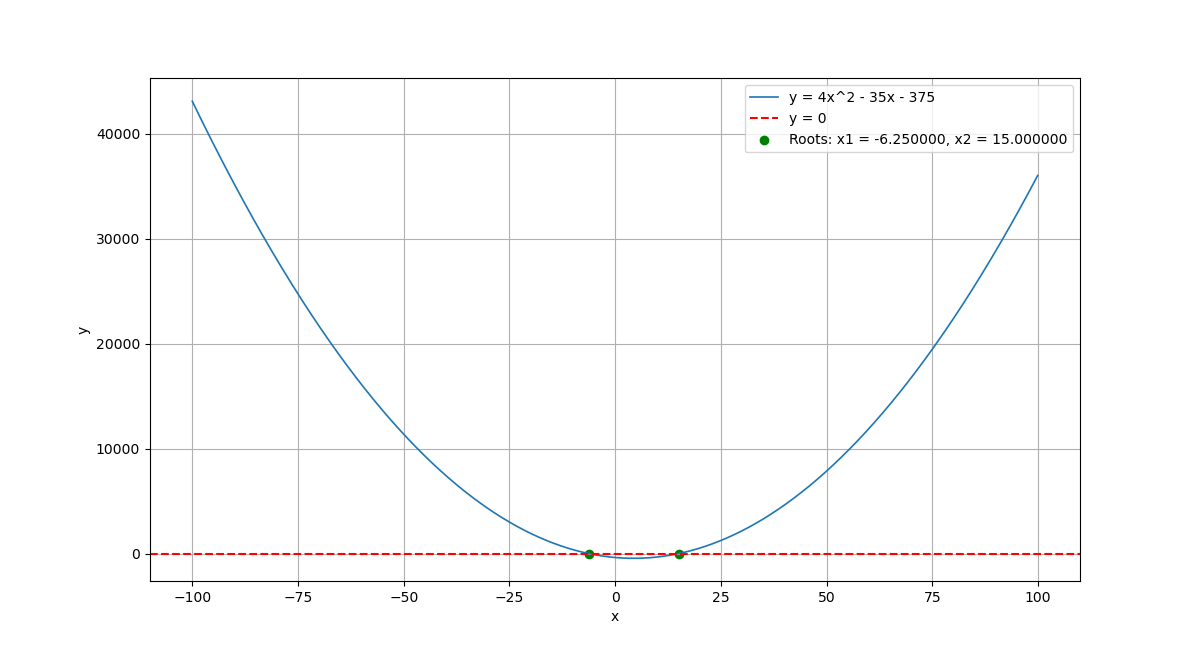
\includegraphics[width=\columnwidth]{figs/Figure_1.png}
    \label{fig:Plot}
    \end{figure}


\end{document}
